
% \begin{frame}{Podstawowe rozwiązania psuedo-rezystorów}


%         \begin{figure}[H]
%             \centering
%             \includegraphics[scale = 0.6]{ch2/ntpr.pdf}

%         \end{figure}
%         \vspace{-5mm} %5mm vertical space
%         % Różne topologie pseudo-rezystorów z niekontrolowaną wartością rezystancji zaimplementowane w przedwzmacniaczu ze sprzężeniem zmiennoprądowym.        
%         \begin{alertblock}{Wady}
%             \begin{itemize}
%                 \item stała rezystancja 
%                 \item brak możliwości regulacji częstotliwości granicznej
%             \end{itemize}
%         \end{alertblock}



% \end{frame}

% \begin{frame}{Podstawowe rozwiązania psuedo-rezystorów - regulowana wartość rezystancji}
%     \begin{block}{}
%         Regulacja częstotliowści granicznej
%     \end{block}

%     \begin{columns}
%         \column{.58\textwidth}
%         \hspace{-10mm} %5mm vertical space
%         \begin{figure}[H]

%             \includegraphics[scale = 0.6]{ch2/tpr.pdf}

%         \end{figure}
%         \column{.35\textwidth}
%         % Różne topologie pseudo-rezystorów z kontrolowaną wartością rezystancji zaimplementowane w przedwzmacniaczu ze sprzężeniem zmiennoprądowym.
%         \vspace{-5mm} \begin{alertblock}{}
%         Zmieniające się napięcie panujące pomiędzy bramką a źródłem tranzystora w zależności od sygnału wejściowego
%         \end{alertblock}
%         \vspace{5mm} 
%         \begin{exampleblock}{}
%             Zachowanie stałego napięcia pomiędzy bramką, a źródłem niezależnie od sygnału wejsciowego 

%         \end{exampleblock}
%     \end{columns}


% \end{frame}


% \begin{frame}{Podstawowe rozwiązania psuedo-rezystorów}
%     \vspace{-1em}
%     \begin{block}{}
%         Zastosowanie tranzystorów jako elementów rezystancjach, zwanych pseudo-rezystorami, jest powszechną praktyką w projektowaniu obwodów analogowych dla przypadków, w których bierne rezystory nie są odpowiednie ze względu na wartości wymaganych rezystancji lub powierzchnie takich elementów. 
%        \end{block}
%     \begin{columns}
%         \column{.48\textwidth}
%         \vspace{-2em}
%         \begin{figure}[H]
%             \includegraphics[scale = 0.4]{ch2/ntpr.pdf}
%         \end{figure}
%         \begin{alertblock}{}
%             Brak możliwości regulacji wartości rezystancji
%         \end{alertblock}

%         \column{.48\textwidth}
%         \vspace{-1em}

%         \begin{figure}[H]
%             \includegraphics[scale = 0.4]{ch2/tpr.pdf}
%         \end{figure}
%         \vspace{-1em}
%         \begin{exampleblock}{}
%             Możliwość regulacji wartości rezystancji za pomocą modyfikacji napięcia panującego na bramce tranzystora
%         \end{exampleblock}

%     \end{columns}
% \end{frame}

% \begin{frame}{Analiza stałoprądowa}

        
%     \vspace{-1em}


%     \begin{columns}
%         \column{.48\textwidth}
%          \begin{alertblock}{}
%             \begin{figure}[H]
%                 \includegraphics[scale=0.8]{ch3/ptune.pdf}
%             \end{figure}
%             \end{alertblock}
%         \column{.48\textwidth}
%         \begin{exampleblock}{}
%             \begin{figure}[H]
%                 \includegraphics[scale=0.8]{ch3/pvgs.pdf}
%             \end{figure}

%         \end{exampleblock}
%     \end{columns}

% \vspace{-0.5em}
%     \begin{columns}
%         \column{.48\textwidth}
%         \begin{figure}[H]
%             \centering
%             \includegraphics[scale = 0.7]{scripts/tmp/pseudoresistors_IV.pdf}
%                 \end{figure}
%         \column{.48\textwidth}
%         \begin{figure}[H]
%             \centering
%             \includegraphics [scale = 0.7]{scripts/tmp/pseudoresistors_R.pdf}
%         \end{figure}
%     \end{columns}


% \end{frame}

\begin{frame}{Architektura wzmacniacza neuronowego wykorzystującego sprzężenie zmiennoprądowe z różnymi implementacjami pseudo-rezystorów}
    \begin{columns}[t]

        \column{.5\textwidth}
        \vspace{-2em} %5mm vertical space

        \begin{alertblock}{Zmieniające się napięcie  pomiędzy bramką a źródłem tranzystora w zależności od sygnału wejściowego: $variable-V_{gs}$}

            \begin{figure}[H]
                \centering
                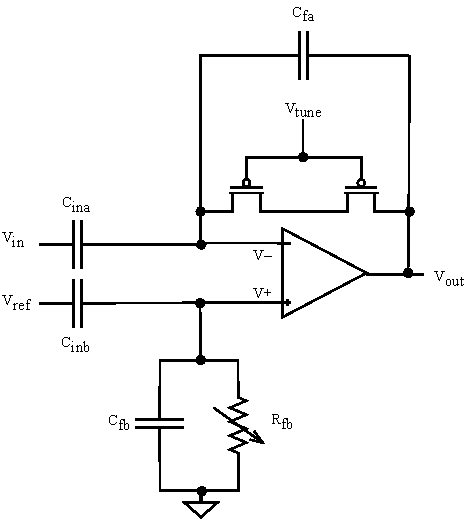
\includegraphics[scale = 0.55]{Figures/standard.pdf}
            \end{figure}
        \end{alertblock}

        \column{.45\textwidth}
        \vspace{-2em} %5mm vertical space

        \begin{exampleblock}{Stałe napięcie pomiędzy bramką, a źródłem niezależnie od sygnału wejsciowego: $fixed-V_{gs}$}
            \begin{figure}[H]
                \centering
                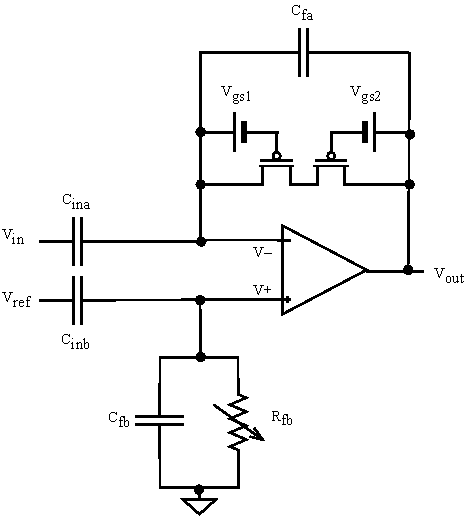
\includegraphics[scale = 0.55]{Figures/project.pdf}
            \end{figure}
        \end{exampleblock}

    \end{columns}
\end{frame}

\begin{frame}{Analiza liniowości pseudo-rezystorów}
    \vspace{-1em}



    \begin{columns}
        \column{.33\textwidth}
        \begin{block}{Modele symulacyjne}
            \begin{itemize}
                \item $variable-V_{gs}$
                 \begin{figure}[H]
                    \centering
                    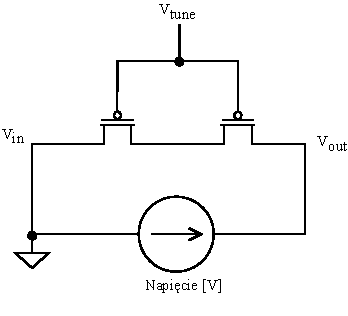
\includegraphics[scale = 0.5]{Figures/standardDC.pdf}
                \end{figure}
                \item $fixed-V_{gs}$
                \begin{figure}[H]
                    \centering
                    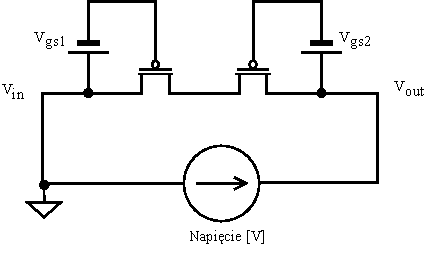
\includegraphics[scale = 0.5]{Figures/projectDC.pdf}
                \end{figure}
            \end{itemize}

\end{block}
        \column{.64\textwidth}
        \begin{itemize}
            \item Badanie odpowiedzi stałoprądowej  
            \item Napięcia polaryzujące bramki tranzystorów dostosowane do ustawień częstotliwości granicznej dla układów ze sprzężeniem AC $\SI{\sim 1}{\hertz}$

            % \item Amplitudy poszczególnych harmonicznych 
        \end{itemize}
    \begin{columns}
    \column{.45\textwidth}

        \begin{figure}[H]
            \centering
            \includegraphics[scale = 0.6]{scripts/tmp/pseudoresistors_IV.pdf}
        \end{figure}

    \column{.45\textwidth}

        \begin{figure}[H]
            \centering
            \includegraphics [scale = 0.6]{scripts/tmp/pseudoresistors_R.pdf}
        \end{figure}

    \end{columns}
\end{columns}


\end{frame}

\begin{frame}{Analiza zniekształceń pseudo-rezystorów}
    \vspace{-1em}
    \begin{columns}
        \column{.33\textwidth}
        \begin{block}{Ustawienia symulacji}
            \begin{itemize}
                \item Badanie odpowiedzi układu  w dziedzinie czasu na wymuszenia sinusoidalne
                \item Częstotliwość graniczna dla układów ze sprzężeniem AC $\SI{\sim 1}{\hertz}$
                \item Analiza: Transformata Fouriera -- wyznaczenie współczynnika THD -- miara liniowości rejestrowanego sygnału
                \item $\mathrm{THD} = \frac{\sqrt{\sum_{n=2}^{+\infty} U_k^2}}{U_1}$
                % \item Amplitudy poszczególnych harmonicznych 
            \end{itemize}
                \end{block}
        \column{.32\textwidth}
        \vspace{-1em} %5mm vertical space
        \begin{alertblock}{$variable-V_{gs}$}
        \begin{figure}[H]
            \centering
            \includegraphics[scale = 0.65]{scripts/tranTHDAmp/tranTHDAmp_ner.pdf}
        \end{figure}
    \end{alertblock}
        \column{.32\textwidth}
        \vspace{-1em} %5mm vertical space
        \begin{exampleblock}{$fixed-V_{gs}$}
        \begin{figure}[H]
            \centering
            \includegraphics[scale = 0.65]{scripts/tranTHDAmp/tranTHDAmp_pr_sim.pdf}
        \end{figure}
    \end{exampleblock}
    \end{columns}

\end{frame}



% \begin{frame}{Projekt przedwzmacniacza z modelem pseudo-rezystora w technologii $\SI{180}{\nano\metre}$  XFAB}
%     \begin{figure}[H]
%         \centering
%         \includegraphics[scale=1.0]{ch3/pseudo-lay.pdf} 

%     \end{figure}


% \end{frame}

% \begin{frame}{Wpływ pojemnościowych prądów bramki pseudo-rezystorów na zniekształcenia  w technologii $\SI{180}{\nano\metre}$}
%     \vspace{-5mm} %5mm vertical space

%     \begin{columns}
%         \column{.3\textwidth}
%         \begin{figure}[H]

%             \includegraphics[trim={0 0.25cm 0 0.25cm}, clip, scale = 0.6]{scripts/tmp/IdsA.pdf}

%         \end{figure}
%         \column{.3\textwidth}
%         \begin{figure}[H]

%             \includegraphics[trim={0 0.25cm 0 0.25cm}, clip, scale = 0.6]{scripts/tmp/IdsB.pdf}

%         \end{figure}
%         \column{.3\textwidth}
%         \begin{figure}[H]

%             \includegraphics[trim={0 0.25cm 0 0.25cm}, clip, scale = 0.6]{scripts/tmp/IgbA.pdf}

%         \end{figure}

%     \end{columns}
%     \vspace{-10mm} %5mm vertical space
%     \begin{columns}
%         \column{.3\textwidth}
%         \begin{figure}[H]

%             \includegraphics[trim={0 0.25cm 0 0.25cm}, clip, scale = 0.6]{scripts/tmp/IgbB.pdf}

%         \end{figure}
%         \column{.3\textwidth}
%         \begin{figure}[H]

%             \includegraphics[trim={0 0.25cm 0 0.25cm}, clip, scale = 0.6]{scripts/tmp/vOut.pdf}

%         \end{figure}
%         \column{.3\textwidth}
%         \begin{figure}[H]

%             \includegraphics[trim={0 0.25cm 0 0.25cm}, clip, scale = 0.6]{scripts/tmp/Igb_diff.pdf}

%         \end{figure}

%     \end{columns}
        



% \end{frame}


% \begin{frame}{Skalowanie zniekształceń z powierzchnią bramki i grubością tlenku tranzystorów tworzących pseudo-rezystory}
%     \begin{columns}
%         \column{.48\textwidth}
%         \begin{block}{Powierzchnia bramki -- technologia $\SI{180}{\nano\metre}$ }
%             \begin{figure}[H]
%                 \centering
%                 \includegraphics[scale = 0.7]{scripts/analyseTran/analyseTranSize.pdf}
%             \end{figure}
%         \end{block}

%         \column{.48\textwidth}
%         \begin{block}{Zależnosć od technologii}
%             \begin{figure}[H]
%                 \centering
%                 \includegraphics[scale = 0.7]{scripts/analyseTran/analyseTranTechnology.pdf}
%             \end{figure}
%         \end{block}


%     \end{columns}

% \end{frame}

% \begin{frame}{Szumy}
%     \vspace{-5mm} %5mm vertical space

%     \begin{columns}
%     \column{.3\textwidth}
%     \begin{figure}[H]
%         \centering
%         \includegraphics[scale=0.5]{ch2/conceptAC_Harrison.pdf} 
%     \end{figure}
%         \column{.3\textwidth}
%         \begin{figure}[H]
%             \centering
%             \includegraphics[scale = 0.5]{scripts/tmp/fig3_R1.pdf}
%         \end{figure}
%         \column{.3\textwidth}
%         \begin{figure}[H]
%             \centering
%             \includegraphics[scale = 0.5]{scripts/tmp/fig3_R2.pdf}
%         \end{figure}
%     \end{columns}

%     \vspace{-5mm} %5mm vertical space


%     \begin{columns}
%         \column{.3\textwidth}
%         \begin{figure}[H]
%             \centering
%             \includegraphics[scale=0.5]{scripts/noiseOutResistors/fig1_R1.pdf}
%         \end{figure}
%         \column{.3\textwidth}
%         \begin{figure}[H]
%             \centering
%             \includegraphics[scale=0.5]{scripts/noiseOutResistors/fig2.pdf}
%         \end{figure}
%     \end{columns}


% \end{frame}


\begin{frame}{Wpływ pojemności wejściowych na szumy i zniekształcenia}
    \begin{columns}
        \column{.49\textwidth}
        \vspace{-1em}

        \begin{figure}[H]
            \centering
            \includegraphics[scale=0.45]{ch2/conceptAC_Harrison.pdf} 
        \end{figure}
\vspace{-2em}

        \begin{block}{Parametry}
            \begin{itemize}
                \item Różne wartości $C_{in}$, oraz $C_{f}$ przy stałym stosunku wzmocnienia $Gain = \SI{20}{\volt\per\volt}$
                \item Wartości $R_{f}$ dostoswane dla każdej symulacji niezależnie tak, aby uzyskać tę samą częstotliwość graniczną $\SI{1}{\hertz}$
                \item Ekwiwalentne szumy wejściowe mierzone w paśmie $\SI{1}{\hertz}$ -- $\SI{10}{\kilo\hertz}$
            \end{itemize}
                \end{block}

            \column{.5\textwidth}
\vspace{-1em}
    \begin{figure}[H]
        \centering
        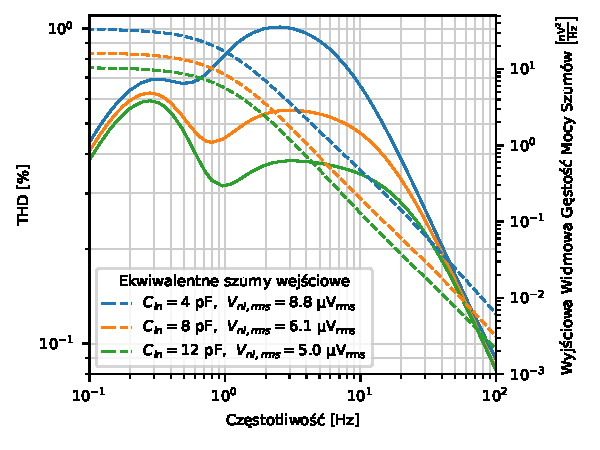
\includegraphics[scale=0.8]{Figures/thd_C_in.pdf} 
    \end{figure}
    \vspace{-2em}

    {\renewcommand\normalsize{\small}%
    \normalsize
    Powierzchnia pojemności $\SI{4}{\pico\farad} \approx\SI{2000}{\micro\metre\squared}$ 
    Powierzchnia pojedynczego przedwzmacniacza (szacunek)  $\approx\SI{7000}{\micro\metre\squared}$ }
\end{columns}

\end{frame}
